\section{Adding a Table of Contents}

Creating a table of contents is straightforward because the command \verb|\tableofcontents| does almost all the work for you:

\begin{tcolorbox}
\begin{verbatim}
    \documentclass{article}
    \title{Sections and Chapters}
    \author{Gubert Farnsworth}
    \date{August 2022}
    \begin{document}
  
    \maketitle
  
    \tableofcontents

    \section{Introduction}
   
    This is the first section.
      
    Lorem  ipsum  dolor  sit  amet,  consectetuer  adipiscing  
    elit.   Etiam  lobortisfacilisis sem.  Nullam nec mi et 
    neque pharetra sollicitudin.  Praesent imperdietmi nec ante. 
    Donec ullamcorper, felis non sodales...
       
    \section*{Unnumbered Section}
    \addcontentsline{toc}{section}{Unnumbered Section}

    Lorem ipsum dolor sit amet, consectetuer adipiscing elit.  
    Etiam lobortis facilisissem.  Nullam nec mi et neque pharetra 
    sollicitudin.  Praesent imperdiet mi necante...

    \section{Second Section}
       
    Lorem ipsum dolor sit amet, consectetuer adipiscing elit.  
    Etiam lobortis facilisissem.  Nullam nec mi et neque pharetra 
    sollicitudin.  Praesent imperdiet mi necante...
    \end{document}
\end{verbatim}
\end{tcolorbox}

This example produces the following output:

\fbox{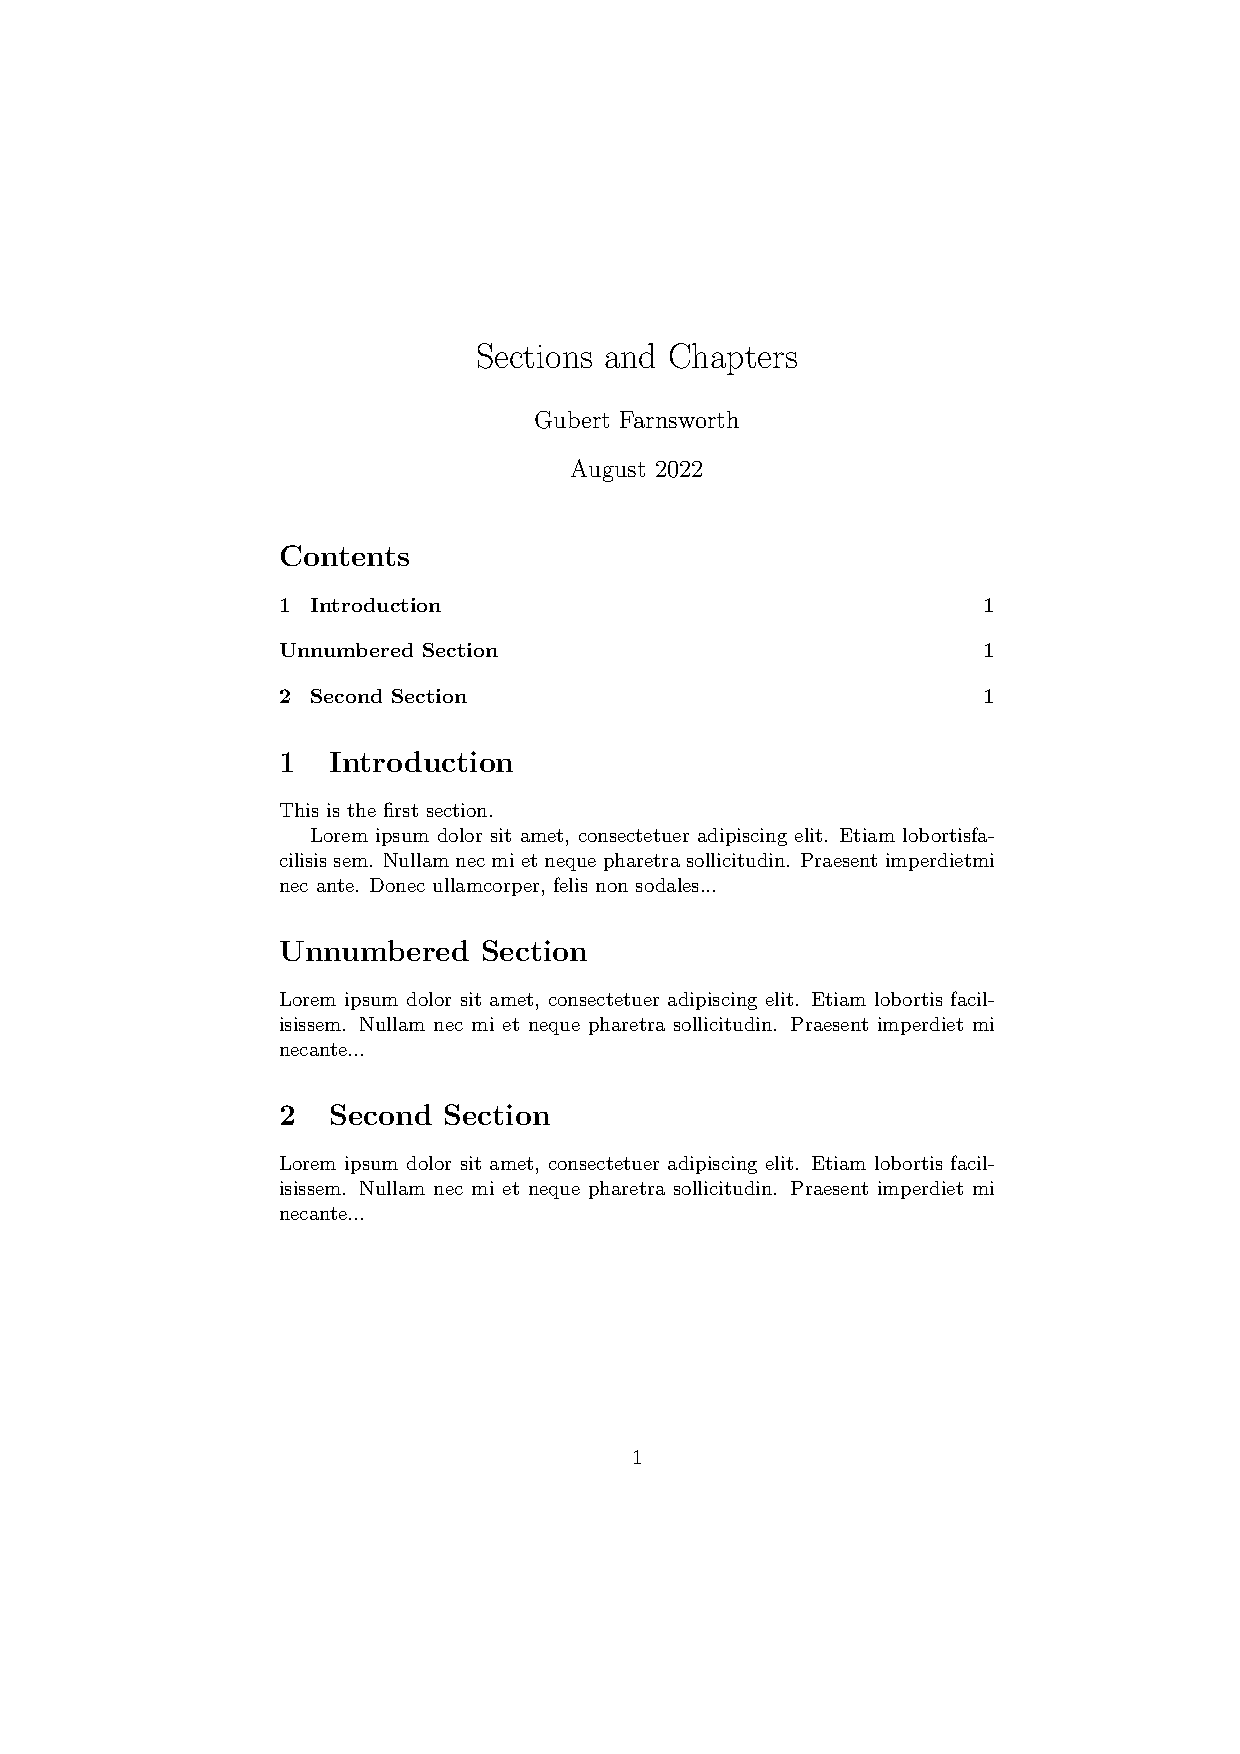
\includegraphics[width=\textwidth]{Example 14-1}}

Sections, subsections and chapters are automatically included in the table of contents. To manually add entries, such as an unnumbered section, use the command \verb|\addcontentsline| as shown in the example.